\documentclass{beamer}
\usetheme{default}
\usepackage[russian]{babel}
\usepackage[utf8]{inputenc}
\usepackage{graphicx}
\begin{document}
\title{Белорусизация cuneiform}
\author{Юрий Адамов \\ AKA \\ begemotv2718}
\date{\today}
\frame{\titlepage}
\begin{frame}{Системы OCR}
\begin{block}{Проприетарные}
\begin{itemize}
\item FineReader
\end{itemize}
\end{block}

\begin{block}{Open source}

\begin{itemize}
\item Tesseract
\item Cuneiform
\item Claraocr
\item gocr
\item \... ?
\end{itemize}
\end{block}
\pause
\begin{block}{Cuneiform}
поддерживает русский, болгарский, сербский, украинский, казахский\...
\end{block}
\end{frame}

\begin{frame}{Как добавлять язык}

\begin{block}{Основная часть} 
тривиальна (добавление языка во всевозможные списки, алфавит кириллический, большая часть сделана для украинского)
\end{block}

\begin{block}{\Large $\breve{y}$} 
 код копируется с русского {\Large й}
\end{block}

\begin{block}{Однако!}
 Есть интересная часть -- словари.
\end{block}
\end{frame}


\begin{frame}{Словарь}
\begin{block}{Программа для генерации словарей}
в самом пакете отсутствует $\to$ Самописная


\end{block}
	
\begin{block}{Формат словарей cuneiform} 

 таблица основ (дерево) + таблица окончаний
\end{block}

\begin{block}{}
нужны слова с таблицей окончаний
\end{block}

\end{frame}

\begin{frame}{Подготовка базы слов}
\begin{block}{Исходный материал}
\begin{itemize}
\item Словарь для ispell
\item Словарь для hunspell (via Ihar Hrachyshka)
\item *Корпус текстов + linguistica*
\item Корпус текстов + (stemka, mystem)
\end{itemize}
\end{block}
\end{frame}
\begin{frame}{Образец относительно хороший}
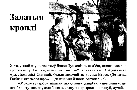
\includegraphics[height=60mm]{sample.pdf}
\end{frame}
\begin{frame}{Образец относительно хороший}

Залатыя 

кроплі

Хата, у якой пэйны час жыў Лявон Луцкевіч зь сям'ею, стаяла пасярод густога лесу. Зрэшты, яе ўсе так і звалі вЂ” "Лясная хатка". А збудаваў яе муж Людзьвікі Сівіцкай, больш вядомай як Зоська Верас. (Яе дачка Галіна й стала спадарожніцай жыцьця Лявона Антонавіча). 
Усе было тут добра: цішыня, якую толькі дапаўняла цвырканьне ды шчэбет птушак, наўкола была некранутая прырода, — працуй, думай, а стаміўся — шчыруй у сваім гародчыку, дзе поўна было розных дзівосаў. Аб цывілізацыі нагадваў толькі далекі водгалас цягнікоў... І цяжка было паверыць, што зусім побач, за гарою, пачынаецца вялікі старажытны горад — Вільня. 

Але жыцьце ч ".Лясной хатцы" ўскладняла адна праблема — не было студні. Як ні шукалі ваду, дзе ні сьвідравалі вЂ” не знаходзілі жылу. А без вады — якое жыцьце. І даводзілася неяк выкручвацца — пітную ваду прывозіць з гораду, а для гаспадарчых мэтаў зьбіраць па кропельцы ўсялякую: і дажджавую, і ад расталага сьнегу. Цэлая сыстэма была распрацаваная, каб найлепш улавіць, захаваць ды як мага рацыянальней выкарыстаць здабытую вадзіцу. 

\end{frame}
\begin{frame}{Образец похуже}

Л 86 

БОК 908 (474.5)

Фотаздымкі

В.Харчаикі', В. Савяикова, В. Бальчуц)са,

А. Кун чуса, М. Сакалаускаса.

ІЯВМ 9986-9228-2-8

© Луцкевіч Лявон, 1993

Выданьне кнігі сыпалася магчымае дзякуючы фі нанспвпй дапамозе

спи. Ялі'иы Кахаиоускаюї, спи. Алены Сіуко-Парасоиене,

спн. Гсиі иы Вой ці к, Фуидацыі П.Крэчэускага.
\end{frame}


\begin{frame}{Где искать}
\begin{center}
begemotv2718.github.com/cuneiform-by
\end{center}
\end{frame}

\end{document}
